\documentclass[11pt,oneside]{article}

\pdfminorversion=7
\usepackage{QuizStyle}

\hypersetup{
    pdftitle={20261118 Quiz for MATH200 Differential Equations},
    pdfauthor={Jungwoo Kim},
    pdfsubject={Quiz for MATH200 Differential Equations},
    pdfcreator={LaTeX}
}

\begin{document}

\quiztitle{20261118 Quiz}

% Boyce Section 5.2, Problem 1; selected subparts (a), (b).
\begin{problem}{5.2.1}
Consider the differential equation
\[
    y''-xy'-y=0,\qquad x_0=1.
\]
\begin{problemsubparts}
    \item Seek power series solutions about $x_0$ and find the recurrence relation satisfied by their coefficients.
    \item Find the first four nonzero terms in each of two solutions $y_1$ and $y_2$ (unless the series terminates sooner).
\end{problemsubparts}
\end{problem}

\begin{solution}
\noindent\textup{(a)} Put $z=x-1$ and seek a solution in the form
\[
    y(x)=\sum_{n=0}^{\infty}a_nz^n.
\]
Since $x=z+1$, substituting into $y''-(z+1)y'-y=0$ gives
\[
    \sum_{n=0}^{\infty}
    (n+1)\left((n+2)a_{n+2}-a_{n+1}-a_n\right)z^n=0.
\]
Thus the recurrence relation is
\[
    \boxed{a_{n+2}=\frac{a_{n+1}+a_n}{n+2}},\qquad n\geq0.
\]

\noindent\textup{(b)} Choose $(a_0, a_1)=(1, 0)$ for $y_1$ and $(a_0, a_1)=(0, 1)$ for $y_2$. Applying the recurrence yields
\[
    \boxed{\begin{aligned}
    y_1(x)&=1+\frac12z^2+\frac16z^3+\frac16z^4+\cdots,\\
    y_2(x)&=z+\frac12z^2+\frac12z^3+\frac14z^4+\cdots,
    \end{aligned}}
    \qquad z=x-1.
\]
Each series displays its first four nonzero terms.
\end{solution}

% Boyce Section 5.2, Problem 2; all subparts (a)--(d).
\begin{problem}{5.2.2}
Consider the differential equation
\[
    y''-xy'-y=0,\qquad x_0=0.
\]
\begin{problemsubparts}
    \item Seek power series solutions about $x_0$ and find the recurrence relation satisfied by their coefficients.
    \item Find the first four nonzero terms in each of two solutions $y_1$ and $y_2$ (unless the series terminates sooner).
    \item By evaluating the Wronskian $W(y_1, y_2)(x_0)$, show that $y_1$ and $y_2$ form a fundamental set of solutions.
    \item If possible, find the general term in each solution.
\end{problemsubparts}
\end{problem}

\begin{solution}
\noindent\textup{(a)} Substitute $y(x)=\sum_{n=0}^{\infty}a_nx^n$ into the equation:
\[
    \sum_{n=0}^{\infty}(n+1)\left((n+2)a_{n+2}-a_n\right)x^n=0.
\]
Therefore
\[
    \boxed{a_{n+2}=\frac{a_n}{n+2}},\qquad n\geq0.
\]

\noindent\textup{(b)} Choosing $(a_0, a_1)=(1, 0)$ and $(0, 1)$, respectively, gives
\[
    \boxed{\begin{aligned}
      y_1(x)&=1+\frac{x^2}{2}+\frac{x^4}{8}+\frac{x^6}{48}+\cdots,\\
      y_2(x)&=x+\frac{x^3}{3}+\frac{x^5}{15}+\frac{x^7}{105}+\cdots.
    \end{aligned}}
\]

\noindent\textup{(c)} The chosen initial coefficients give $y_1(0)=1$, $y_1'(0)=0$, $y_2(0)=0$, and $y_2'(0)=1$. Hence
\[
    \boxed{W(y_1, y_2)(0)=
    \begin{vmatrix}1&0\\0&1\end{vmatrix}=1\ne0}.
\]
Thus $y_1$ and $y_2$ are linearly independent and form a fundamental set of solutions.

\noindent\textup{(d)} Iterating the recurrence separately for even and odd indices gives
\[
    a_{2n}=\frac{a_0}{2^n n!},\qquad
    a_{2n+1}=\frac{a_1}{(2n+1)!!},\qquad n\geq0,
\]
where $(2n+1)!!=1\cdot3\cdots(2n+1)$. Consequently,
\[
    \boxed{\begin{aligned}
      y_1(x)&=\sum_{n=0}^{\infty}\frac{x^{2n}}{2^n n!},\\
      y_2(x)&=\sum_{n=0}^{\infty}\frac{x^{2n+1}}{(2n+1)!!}.
    \end{aligned}}
\]
\end{solution}

% Boyce Section 5.3, Problem 4.
\begin{problem}{5.3.4}
Determine a lower bound for the radius of convergence of series solutions of
\[
    y''+4y'+6xy=0
\]
about each of the points $x_0=0$ and $x_0=3$.
\end{problem}

\begin{solution}
In standard form the coefficients $p(x)=4$ and $q(x)=6x$ are entire. There are no finite singular points, so the series solutions centered at either ordinary point converge for all real $x$ (indeed, for all complex $x$). Thus
\[
    \boxed{R=\infty\quad\text{for }x_0=0\text{ and }x_0=3}.
\]
\end{solution}

% Boyce Section 5.3, Problem 5.
\begin{problem}{5.3.5}
Determine a lower bound for the radius of convergence of series solutions of
\[
    (x^2-2x-3)y''+xy'+4y=0
\]
about $x_0=5$, $x_0=-5$, and $x_0=0$.
\end{problem}

\begin{solution}
The coefficients in standard form are
\[
    p(x)=\frac{x}{(x-3)(x+1)},\qquad
    q(x)=\frac{4}{(x-3)(x+1)}.
\]
Their singular points are $x=3$ and $x=-1$. The distance from each center to the nearest singular point gives the guaranteed radius:
\[
    \begin{aligned}
      x_0=5:&\quad R\geq\min(2, 6)=\boxed{2},\\
      x_0=-5:&\quad R\geq\min(8, 4)=\boxed{4},\\
      x_0=0:&\quad R\geq\min(3, 1)=\boxed{1}.
    \end{aligned}
\]
\end{solution}

% Boyce Section 5.3, Problem 6.
\begin{problem}{5.3.6}
Determine a lower bound for the radius of convergence of series solutions of
\[
    xy''+y=0
\]
about $x_0=2$.
\end{problem}

\begin{solution}
Dividing by $x$ gives $y''+y/x=0$, whose only finite singular point is $x=0$. Its distance from the center $x_0=2$ is $2$. Hence the theorem guarantees
\[
    \boxed{R\geq2}.
\]
\end{solution}

% Boyce Section 5.3, Problem 8.
\begin{problem}{5.3.8}
For the differential equation
\[
    e^xy''+xy=0,
\]
find the first four nonzero terms in each of two power series solutions about the origin. Show that they form a fundamental set of solutions. What do you expect the radius of convergence to be for each solution?
\end{problem}

\begin{solution}
Dividing by $e^x$ gives $y''+xe^{-x}y=0$. Write
\[
    y=\sum_{n=0}^{\infty}a_nx^n,
    \qquad xe^{-x}=\sum_{k=1}^{\infty}\frac{(-1)^{k-1}}{(k-1)!}x^k.
\]
Equating coefficients yields
\[
    (n+2)(n+1)a_{n+2}
      +\sum_{k=1}^{n}\frac{(-1)^{k-1}}{(k-1)!}a_{n-k}=0,
    \qquad n\geq0.
\]
Taking $(a_0, a_1)=(1, 0)$ and $(0, 1)$ gives
\[
    \boxed{\begin{aligned}
      y_1(x)&=1-\frac{x^3}{6}+\frac{x^4}{12}-\frac{x^5}{40}+\cdots,\\
      y_2(x)&=x-\frac{x^4}{12}+\frac{x^5}{20}-\frac{x^6}{60}+\cdots.
    \end{aligned}}
\]
Since $W(y_1, y_2)(0)=1$, these solutions form a fundamental set. Both coefficients in the standard equation, $0$ and $xe^{-x}$, are entire, so the radius of convergence of each series is
\[
    \boxed{R=\infty}.
\]
\end{solution}

% Boyce Section 5.4, Problem 1.
\begin{problem}{5.4.1}
Find the general solution of
\[
    x^2y''+5xy'+3y=0
\]
valid on any interval not containing the singular point.
\end{problem}

\begin{solution}
For the Euler equation, set $y=x^r$ on $x>0$. The indicial equation is
\[
    r(r-1)+5r+3=(r+1)(r+3)=0.
\]
The two power functions also solve the equation for $x<0$, giving
\[
    \boxed{y(x)=c_1x^{-1}+c_2x^{-3}},\qquad x\ne0,
\]
with arbitrary constants on each interval not containing $0$.
\end{solution}

% Boyce Section 5.4, Problem 3.
\begin{problem}{5.4.3}
Find the general solution of
\[
    x^2y''-5xy'+9y=0
\]
valid on any interval not containing the singular point.
\end{problem}

\begin{solution}
The indicial equation
\[
    r(r-1)-5r+9=(r-3)^2=0
\]
has the repeated root $r=3$. The Euler equation therefore has the general solution
\[
    \boxed{y(x)=x^3(c_1+c_2\ln|x|)},\qquad x\ne0,
\]
on any interval not containing $0$.
\end{solution}

% Boyce Section 5.4, Problem 4.
\begin{problem}{5.4.4}
Find the general solution of
\[
    x^2y''+3xy'+10y=0
\]
valid on any interval not containing the singular point.
\end{problem}

\begin{solution}
The indicial equation is
\[
    r(r-1)+3r+10=r^2+2r+10=0,
\]
whose roots are $r=-1\pm3i$. Therefore
\[
    \boxed{y(x)=|x|^{-1}\left(c_1\cos(3\ln|x|)
          +c_2\sin(3\ln|x|)\right)},\qquad x\ne0.
\]
The constants are chosen independently on each interval not containing $0$.
\end{solution}

% Boyce Section 5.4, Problem 8.
\begin{problem}{5.4.8}
Find the general solution of
\[
    (x-1)^2y''+8(x-1)y'+12y=0
\]
valid on any interval not containing the singular point.
\end{problem}

\begin{solution}
Set $z=x-1$. The equation becomes $z^2y''+8zy'+12y=0$, with indicial equation
\[
    r(r-1)+8r+12=(r+3)(r+4)=0.
\]
Thus
\[
    \boxed{y(x)=c_1(x-1)^{-3}+c_2(x-1)^{-4}},\qquad x\ne1,
\]
on any interval not containing $1$.
\end{solution}

% Boyce Section 5.4, Problem 11.
\begin{problem}{5.4.11}
Solve the initial value problem
\[
    x^2y''-3xy'+4y=0,\qquad y(-1)=2,\qquad y'(-1)=2.
\]
Plot the graph of the solution and describe its behavior as $x\to0$.
\end{problem}

\begin{solution}
The indicial equation is
\[
    r(r-1)-3r+4=(r-2)^2=0.
\]
As the initial point is $-1$, the relevant interval is $x<0$, on which
\[
    y=x^2(c_1+c_2\ln(-x)).
\]
From $y(-1)=c_1=2$ and $y'(-1)=-2c_1-c_2=2$, we obtain $c_2=-6$. Hence
\[
    \boxed{y(x)=x^2(2-6\ln(-x))},\qquad x<0.
\]
Since $x^2\ln(-x)\to0$ as $x\to0^-$, the solution approaches zero:
\[
    \boxed{\lim_{x\to0^-}y(x)=0}.
\]
The graph is shown below, with an open circle at $x=0$ because the differential equation is singular there.
\begin{center}
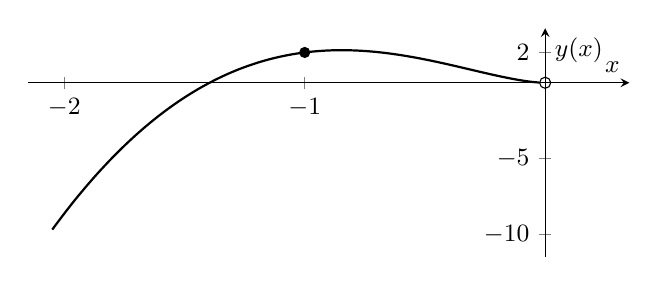
\begin{tikzpicture}
\begin{axis}[
    width=0.76\textwidth,
    height=0.37\textwidth,
    axis lines=middle,
    xmin=-2.15, xmax=0.35,
    ymin=-11.5, ymax=3.6,
    xlabel={$x$}, ylabel={$y(x)$},
    xtick={-2,-1,0},
    ytick={-10,-5,0,2},
    tick label style={font=\small},
    label style={font=\small},
    clip=false,
    samples=250
]
    \addplot[black,thick,domain=-2.05:-0.025] {x^2*(2-6*ln(-x))};
    \addplot[only marks,mark=*,mark size=1.8pt,black] coordinates {(-1,2)};
    \addplot[only marks,mark=o,mark size=2pt,black] coordinates {(0,0)};
\end{axis}
\end{tikzpicture}
\end{center}
\end{solution}

\end{document}
